\documentclass[tikz, border=1mm]{standalone}

%% FEYNMAN DIAGRAMS
\usepackage[compat=1.1.0]{tikz-feynman}
\tikzfeynmanset{warn luatex=false}

\begin{document}
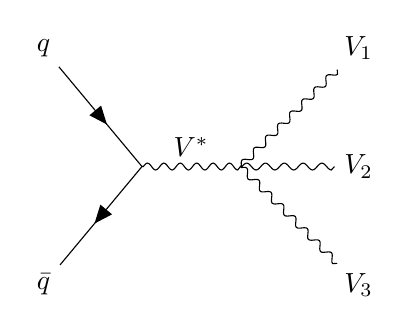
\begin{tikzpicture}
  \begin{feynman}
    \vertex (i1) at (0,3) {\(q\)};
    \vertex (i2) at (0,0) {\(\bar{q}\)};
    \vertex (a)  at (1.25,1.5);
    \vertex [right=1.25 of a] (b);
    \vertex (f1) at (4,3) {\(V_{1}\)};
    \vertex [below=1.5 of f1] (f2) {\(V_{2}\)};
    \vertex [below=1.5 of f2] (f3) {\(V_{3}\)};

    \diagram* {
      (i1) -- [fermion] (a) -- [fermion] (i2),
      (a) -- [boson, edge label=\(V^{*}\)] (b),
      (b) -- [boson] (f1),
      (b) -- [boson] (f2),
      (b) -- [boson] (f3),
    };
  \end{feynman}
\end{tikzpicture}
\end{document}
